\documentclass{article}

% NeurIPS 2026
% \usepackage{neurips_2026}
\usepackage[nonanonymous]{neurips_2026}

\usepackage[utf8]{inputenc}
\usepackage[T1]{fontenc}
\usepackage{hyperref}
\usepackage{url}
\usepackage{booktabs}
\usepackage{amsfonts}
\usepackage{amsmath}
\usepackage{nicefrac}
\usepackage{microtype}
\usepackage{xcolor}
\usepackage{graphicx}
\usepackage{subcaption}
% Figures are pre-rendered PDFs in figures/ produced by Plotly + kaleido.
% The Python source that builds them is figures/make_figures.py.

\title{Sequence, Structure, or Both?\\
A GAT Ablation for Multi-Label Protein Subcellular Localization}

\author{%
  Ashwin Ajai\\
  Department of Computer Science\\
  Virginia Tech\\
  Blacksburg, VA 24061\\
  \texttt{ashwinajai12@gmail.com}\\
  \And
  Saksham Kumar\\
  Department of Computer Science\\
  Virginia Tech\\
  Blacksburg, VA 24060\\
  \texttt{sakshamkumar@vt.edu}\\
}

\begin{document}

\maketitle

\begin{abstract}
Protein subcellular localization is a multi-label classification
problem with severe class imbalance: on the homology-controlled
DeepLoc~2.0 split, the rarest of ten compartments (Peroxisome) accounts
for only $1\%$ of the test set while the most abundant (Nucleus)
accounts for $37\%$. We run a controlled five-row ablation that adds
one source of representational power at a time: classical
hand-engineered features, a mean-pooled ESM2-150M embedding fed to an
MLP, a graph attention network (GAT) on sequence-only edges, the same
GAT on AlphaFold-derived $C_\alpha$ contact edges, and a tuned GAT that
uses both edge types. The dominant gain is from swapping hand features
for frozen ESM2 embeddings, which lifts macro test ROC-AUC from $0.812$
to $0.913$. Adding graph structure contributes a further $+0.014$
ROC-AUC and, more importantly, a $+0.07$ improvement in PR-AUC and
$+0.09$ in macro F1 --- gains concentrated on the rare classes. Sequence
and contact edges are near-identical in isolation, but combining them
under a tuned configuration delivers the best PR-AUC ($0.673$) and F1
($0.587$), and lifts Peroxisome PR-AUC nearly $9\times$ over the
classical baseline. Using GNNExplainer and raw GATv2 attention on the
headline checkpoint, we find that the model recovers the Peroxisome
PTS1 motif in $45.7\%$ of explained true positives and the mitochondrial
N-terminal targeting region in $30\%$, but does not recover the ER KDEL
motif or plastid N-terminal targeting, providing a clear picture of
which aspects of known biology the network does and does not capture.
\end{abstract}

% =========================================================================
\section{Introduction}\label{sec:intro}
% =========================================================================

A protein's amino-acid sequence carries enough information to predict the
compartment it ends up in, but the relationship is not local: a single
C-terminal tripeptide can route a peroxisomal protein, while
mitochondrial targeting is encoded in a 30--70 residue cleavable
N-terminal pre-sequence whose statistical signature is diffuse rather
than motif-like. This combination of (a) a short, easy-to-learn pattern
for some compartments and (b) a long, distributed signal for others is
why classical $k$-mer or AA-composition classifiers plateau around macro
ROC-AUC $\approx 0.81$ on DeepLoc~2.0, even with nonlinear models.
Two recent developments have changed what is possible without retraining
a large model: the release of frozen protein language model embeddings
(ESM2) that condense pretraining over 65M sequences into a 640-d
per-residue feature, and the public release of AlphaFoldDB, which gives
a predicted structure for every UniProt accession at no inference cost.

This paper asks a focused empirical question: \emph{given frozen
ESM2 embeddings as the per-residue feature, how much additional value
do AlphaFold-derived contact edges contribute on top of the
residue-chain backbone under a fixed, modest compute budget?} We answer by
running a five-row ablation on the leakage-controlled DeepLoc~2.0
split, with a fixed test set held out across all rows, and we
audit the resulting tuned GAT with GNNExplainer to ask whether its
attention recovers known sorting motifs.

\paragraph{Contributions.}
\begin{enumerate}
\item \textbf{A controlled five-row ablation} (Table~\ref{tab:ablation},
Figure~\ref{fig:ablation}) that decomposes the gain from hand features
$\to$ frozen ESM2 $\to$ structure-aware GAT $\to$ tuned GAT with
edge-type embedding, on a single homology-controlled split.
\item \textbf{An edge-type comparison}: GAT-sequence-only and
GAT-contact-only are within $0.002$ macro ROC-AUC of each other, but
combining both under a small random search delivers the best PR-AUC and
F1, suggesting the two edge types carry partially complementary signal.
\item \textbf{An interpretability audit} of the headline GAT with
GNNExplainer and raw GATv2 attention, recovering Peroxisome PTS1 in
$45.7\%$ of explained true positives and mitochondrial N-terminal
targeting in $30\%$, while reporting two null results (ER KDEL and
plastid N-terminal).
\item \textbf{A fully reproducible pipeline}: every stage is exposed
as a \texttt{make gnn-*} target with a fixed seed, and the entire run
completes on a single consumer GPU (8\,GB VRAM) in under two GPU-days.
\end{enumerate}

% =========================================================================
\section{Related Work}\label{sec:related}
% =========================================================================

\paragraph{Subcellular localization predictors.}
Classical predictors such as TargetP and SignalP read the N-terminus
with hand-crafted position-specific scoring matrices; later methods
including LocTree3 and DeepLoc~1 use shallow neural networks on
hand-engineered features. DeepLoc~2.0 is the current gold-standard
benchmark and uses a homology-aware split (sequence identity $\le 30\%$
between train and test) so leakage cannot be hidden by similar protein
families. Our classical baseline panel sits in this lineage.

\paragraph{Pretrained protein representations.}
ESM2~[2] learns per-residue embeddings via masked language
modelling on tens of millions of sequences and has been shown to
linearise structurally and functionally meaningful information in its
hidden states. We use the 150M-parameter checkpoint, frozen, as a
deterministic feature extractor; this is the single largest source of
gain in our ablation.

\paragraph{Structure-aware models.}
AlphaFold~2~[3] provides a high-quality predicted
structure for essentially every UniProt entry. We treat the AlphaFoldDB
as a static lookup, building $C_\alpha$ contact graphs at an 8\,\AA{}
threshold rather than running structure prediction at training time.
Graph attention networks~[5,6] are a natural
fit when the input is a labelled graph with continuous edge attributes;
GATv2 fixes the rank-deficient attention of the original GAT and is what
we use throughout.

\paragraph{Interpretability for graph models.}
GNNExplainer~[7] learns a per-instance soft mask
over node and edge features to identify the smallest sub-graph that
preserves the model's prediction. We use it on high-confidence true
positives from the headline GAT, complemented by raw GATv2 attention,
to ask whether the network's importance map overlaps with canonical
sorting motifs.

% =========================================================================
\section{Methodology}\label{sec:method}
% =========================================================================

\paragraph{Task.}
Multi-label classification: each protein is labelled with a subset of the
ten DeepLoc~2.0 compartments (Cytoplasm, Nucleus, Extracellular, Cell
membrane, Mitochondrion, Plastid, Endoplasmic reticulum, Lysosome /
Vacuole, Golgi apparatus, Peroxisome). We learn a single shared
representation and predict ten sigmoid logits jointly, optimised with
binary cross-entropy plus per-class positive-weight rebalancing
(Eq.~\ref{eq:loss}).

\paragraph{Pipeline overview.}
Figure~\ref{fig:pipeline} shows the full data flow. Per-residue features
come from the frozen ESM2-150M encoder (640-d, fp16, computed once and
cached). Per-protein structure comes from AlphaFoldDB, downloaded by
UniProt accession; we extract $C_\alpha$ coordinates and build two edge
sets, sequence adjacency ($i \leftrightarrow i\!\pm\!1$) and contact
($\|\Delta C_\alpha\| < 8\,\text{\AA}$, off-diagonal). Edges carry a
two-dimensional one-hot edge-type vector that the GAT consumes via
\texttt{edge\_dim=2}.

\begin{figure}[t]
  \centering
  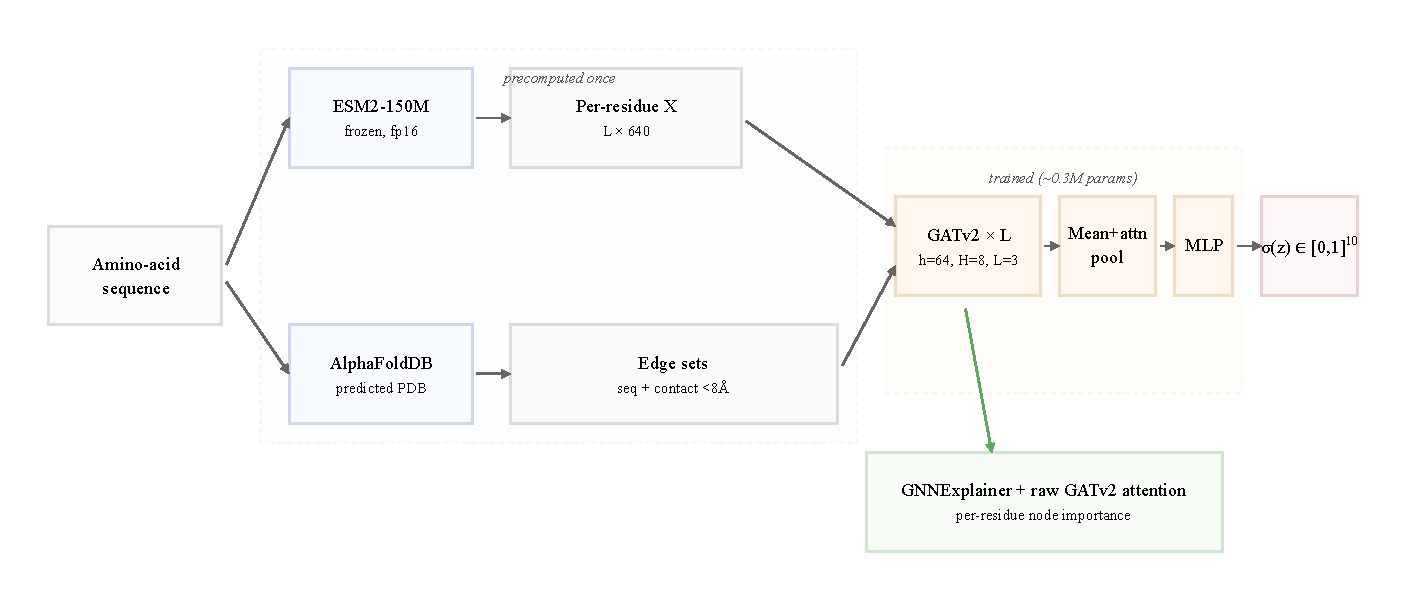
\includegraphics[width=\linewidth]{figures/fig1_pipeline.pdf}
  \caption{Pipeline. Frozen blocks (blue) compute per-residue ESM2
  embeddings and per-protein contact graphs once, and are reused across
  all ablation rows. Trained blocks (orange) total roughly 0.3M
  parameters in the headline configuration. GNNExplainer and raw GATv2
  attention (green) operate post-hoc on the trained headline checkpoint.}
  \label{fig:pipeline}
\end{figure}

\paragraph{Architecture.}
Let $X \in \mathbb{R}^{L\times 640}$ be the per-residue ESM2 embedding,
$E \in \{0,1\}^{2 \times |E|}$ the edge index, and $T \in \{0,1\}^{|E|
\times 2}$ the one-hot edge-type tensor. The GAT applies $L_{\text{layer}}$
GATv2 layers $f^{(\ell)}_{\theta}$ with hidden width $h$ and $H$ heads,
projects to a graph-level vector via concatenated mean and
attention-pooling, and feeds an MLP head:
\begin{equation}
H^{(\ell)} = f^{(\ell)}_{\theta}\!\left(H^{(\ell-1)}, E, T\right),\quad
H^{(0)} = X,\quad
\hat{y} = \sigma\!\Big(\mathrm{MLP}\big[\mathrm{mean}(H^{(L)}),\,
\mathrm{attn}(H^{(L)})\big]\Big).
\label{eq:arch}
\end{equation}
The headline configuration chosen by our random search has
$L_{\text{layer}}{=}3$, $h{=}64$, $H{=}8$, dropout $0$, learning rate
$10^{-3}$. The MeanPool-MLP ablation row substitutes $\hat y =
\sigma(\mathrm{MLP}(\mathrm{mean}_i X_i))$ and uses no graph at all.

\paragraph{Loss.}
With per-class positive rate $\pi_c = N^+_c / N$ from the training set,
the per-class positive weight is $w_c = (1-\pi_c)/\pi_c$, and the loss
for prediction $\hat y \in [0,1]^{10}$ against label $y \in \{0,1\}^{10}$ is
\begin{equation}
\mathcal{L}(\hat y, y) \;=\; -\frac{1}{10}\sum_{c=1}^{10}\Big[
w_c\, y_c \log \hat y_c \;+\; (1-y_c) \log(1-\hat y_c)\Big].
\label{eq:loss}
\end{equation}
This rebalancing is what drives the macro-F1 jump on rare classes
(Section~\ref{sec:results}).

\paragraph{Interpretability.}
On the headline checkpoint we sample up to 50 high-confidence true
positives per compartment. For each, GNNExplainer is run with default
node-feature and edge masks; the resulting per-residue importance is
combined with the layer-averaged GATv2 attention, and we test for
overlap with three known motif templates: PTS1 (\texttt{[SAC]K[LMI]\$})
for Peroxisome, KDEL (\texttt{[KH]DEL\$}) for ER, and ``top-decile of
importance lies in the first 70 residues'' for Mitochondrion and Plastid
N-terminal targeting.

% =========================================================================
\section{Experiments}\label{sec:experiments}
% =========================================================================

\paragraph{Data.}
DeepLoc~2.0, with the homology-controlled split shipped by the dataset
authors: $17{,}145$ train, $5{,}696$ validation, $5{,}462$ test
proteins. The split guarantees that no protein in train shares
$>30\%$ sequence identity with any test protein. After filtering out
proteins for which AFDB has no predicted structure (or the structure
length disagrees with the sequence length post-cleaning), the GNN rows
operate on $16{,}871$ train, $5{,}617$ validation, $5{,}380$ test.
The MLP-pool row does not depend on AlphaFold and uses the full
unfiltered split.

\paragraph{Baselines and rows.}
Row~1 (classical) is a panel of three sklearn classifiers --- logistic
regression, random forest, and an MLP --- each tuned by
\texttt{GridSearchCV} with stratified 5-fold CV on a 30-d
hand-engineered feature vector (length, AA composition, mean
physico-chemistry, sequence entropy, neighbour statistics). Rows 2--4
fix the residue feature to frozen ESM2 and vary only the inductive
bias: row 2 is mean-pool + MLP (no graph), row 3 is GAT on sequence
edges, row 4 is GAT on contact edges. Row 5 is the tuned headline GAT
on both edge types, with hyperparameters chosen by an 8-config random
search (Table~\ref{tab:hyper}, Figure~\ref{fig:sweep}) and refit once on
\texttt{train}\,$\cup$\,\texttt{val} before a single test evaluation.

\paragraph{Optimisation.}
AdamW with cosine schedule, weight decay $10^{-4}$, AMP enabled, batch
size 16 (32 for the MLP-pool row), 20 ablation epochs / 30 headline
epochs / 12 sweep epochs per config. Best epoch is selected by macro
val ROC-AUC; the test set is touched exactly once per row.

\paragraph{Metrics.}
For each label we report ROC-AUC, average precision (PR-AUC), and F1 at
threshold 0.5; macros are unweighted means across the ten compartments.
We treat PR-AUC as the primary metric given the level of class imbalance.

\paragraph{Compute.}
All experiments are run on a single consumer GPU with 8\,GB of VRAM.
End-to-end wall-clock: approximately $2$\,h to download AlphaFoldDB
structures (network-bound, executed in parallel with embedding),
$4$\,h to cache ESM2 embeddings, $1$\,h for graph construction,
$13$\,h for the three ablation rows, $8$\,h for the 8-configuration
random search, $2$\,h for the headline refit, and $1$\,h for
GNNExplainer on 500 proteins.

% =========================================================================
\section{Results}\label{sec:results}
% =========================================================================

\subsection{Ablation table}

\begin{table}[t]
  \caption{Five-row ablation on the DeepLoc~2.0 test set, macro across
  ten compartments. The largest single gain (\textbf{+0.10 ROC-AUC}) is
  from swapping hand-engineered features for frozen ESM2 embeddings,
  before any graph structure is added. Adding sequence or contact
  graph structure adds a further $\sim\!0.014$ in ROC-AUC and meaningful
  jumps in PR-AUC and F1. The tuned headline does not win on ROC-AUC
  but takes the top spot in PR-AUC and F1, which are what matter on
  rare classes.}
  \label{tab:ablation}
  \centering
  \small
  \begin{tabular}{llccc}
    \toprule
    Row & Model & ROC-AUC & PR-AUC & F1 \\
    \midrule
    1   & Classical (random forest, hand features) & 0.8123 & 0.376 & 0.199 \\
    2   & Mean-ESM2 + MLP (no graph)               & 0.9134 & 0.608 & 0.497 \\
    3   & GAT, sequence edges only                 & 0.9226 & 0.644 & 0.563 \\
    4   & GAT, $C_\alpha$ contact edges only       & \textbf{0.9246} & 0.653 & 0.561 \\
    5   & \textbf{GAT, both edges (tuned, headline)} & 0.9211 & \textbf{0.673} & \textbf{0.587} \\
    \bottomrule
  \end{tabular}
\end{table}

\begin{figure}[t]
  \centering
  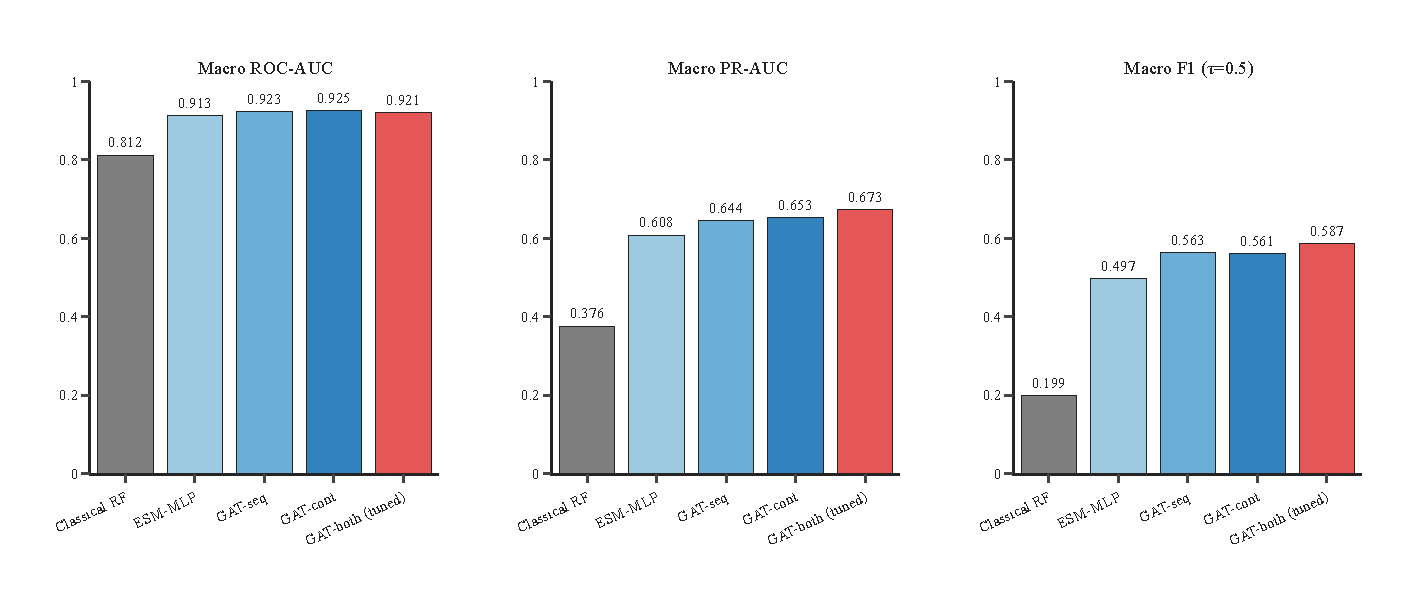
\includegraphics[width=\linewidth]{figures/fig2_ablation.pdf}
  \caption{Macro test metrics across the five ablation rows. The classical
  bar is the best of three sklearn classifiers (random forest). PR-AUC and
  F1 widen the gap between the headline GAT (red) and the simpler
  ablations more than ROC-AUC does, because they respond to the rare-class
  predictions that the BCE positive-weight reweighting fixes.}
  \label{fig:ablation}
\end{figure}

\subsection{Per-compartment behaviour}

The macro numbers compress a wide spread. Figure~\ref{fig:heatmap} shows
ROC-AUC for every (model, compartment) cell. Three patterns are
visible: (i) the row-wise jump from the classical block to the ESM2
block is largest for compartments where the classical model already
struggled (Cell membrane, Cytoplasm), and is smallest for compartments
where it was already strong (Plastid, Extracellular); (ii) once ESM2 is
in play, all four neural rows are within $\sim\!0.02$ of one another on
every compartment, even though F1 disagrees more sharply (see
Section~\ref{sec:f1});  (iii) Lysosome and Golgi remain the hardest
compartments under every model, which is consistent with how diffuse
their sorting signal is in the underlying biology.

\begin{figure}[t]
  \centering
  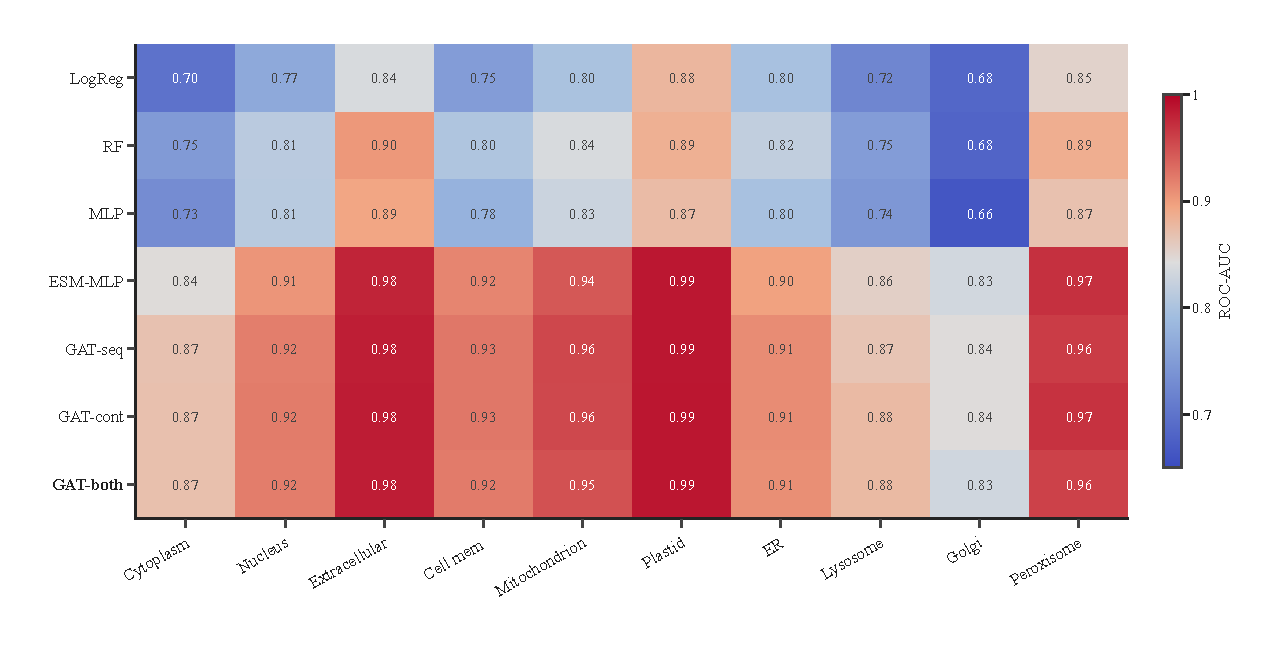
\includegraphics[width=\linewidth]{figures/fig3_heatmap.pdf}
  \caption{Per-(model, compartment) test ROC-AUC. The classical block
  (LogReg, RF, MLP, top) sits in the cooler half of the colormap;
  switching to frozen ESM2 (ESM-MLP and below) shifts the entire row
  warmer, particularly for Cell membrane, Endoplasmic reticulum, and
  Lysosome. Plastid and Extracellular saturate near $0.99$ for every
  neural row. The headline \textbf{GAT-both} is the bottom row.}
  \label{fig:heatmap}
\end{figure}

\begin{figure}[t]
  \centering
  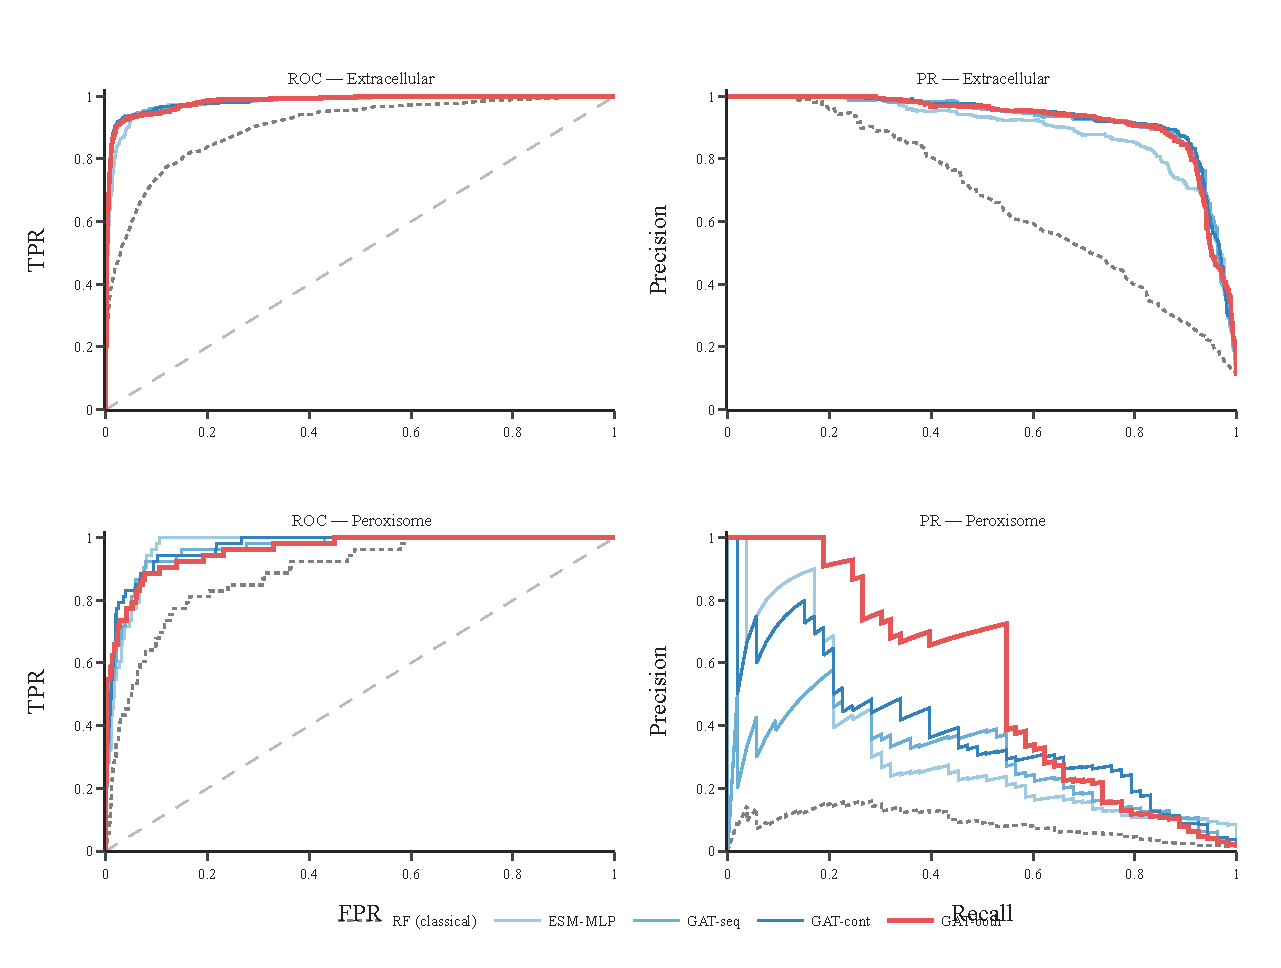
\includegraphics[width=0.95\linewidth]{figures/fig6_curves.pdf}
  \caption{ROC and PR curves for two illustrative compartments.
  Extracellular is an easy compartment ($n_{+}{=}594$) where every
  ESM2-based row tracks the same near-saturated curve. Peroxisome is the
  rarest compartment ($n_{+}{=}53$); the gap between the classical RF
  baseline (gray, dotted) and the headline GAT-both (red, thick) is
  most visible on the PR curve, where the GAT keeps high precision out
  to recall $\sim\!0.6$ while the classical curve collapses early.}
  \label{fig:curves}
\end{figure}

\subsection{F1 under class imbalance and the effect of positive-weight rebalancing}\label{sec:f1}

The classical RF baseline achieves macro F1 of only $0.199$ despite a
perfectly respectable macro ROC-AUC of $0.812$. The reason is sharp:
on the three rarest compartments (Lysosome, Golgi, Peroxisome) the
default 0.5 decision threshold sits above the median positive-class
score, even though \texttt{class\_weight="balanced"} rebalances the loss
during training. Per-class F1 on those three compartments under the
classical RF is $\{0.008,\, 0.000,\, 0.000\}$. The headline GAT, trained
with explicit per-class positive weights $w_c = (1{-}\pi_c)/\pi_c$ in
the BCE loss (Eq.~\ref{eq:loss}), recovers $\{0.298,\, 0.241,\, 0.335\}$
on the same three compartments. PR-AUC tells the same story even more
clearly: classical Peroxisome PR-AUC is $0.060$; the headline GAT lifts
it to $0.536$, a $\sim\!9\times$ jump.

\subsection{Random search and the marginal effect of tuning}

\begin{figure}[t]
  \centering
  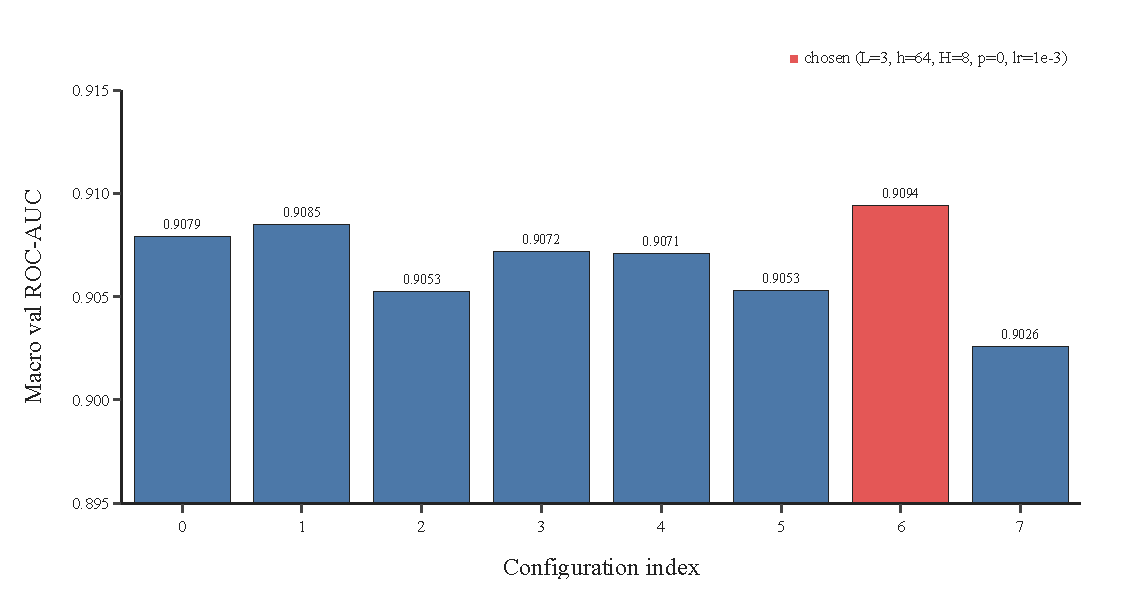
\includegraphics[width=0.85\linewidth]{figures/fig4_sweep.pdf}
  \caption{Eight random-search configurations (12 epochs each, fixed
  seed, sampled from $L \in \{2,3\}, h \in \{64,128\}, H \in \{4,8\},
  p \in \{0,0.2\}, \eta \in \{10^{-3}, 3\!\cdot\!10^{-4}\}$). The
  validation ROC-AUC band is narrow ($0.9026$--$0.9094$, $\Delta\!\approx\!0.7$
  points), which is consistent with a robust architecture and a small
  signal-to-noise ratio in the search; we proceed with the best (red)
  for the headline refit.}
  \label{fig:sweep}
\end{figure}

\begin{table}[t]
  \caption{Headline configuration chosen by random search (val
  ROC-AUC = 0.9094). The fact that ROC-AUC is nearly flat across the
  eight configurations is itself a finding: this architecture is
  robust to depth, width, head count, dropout, and learning rate within
  the tested ranges.}
  \label{tab:hyper}
  \centering
  \small
  \begin{tabular}{lc}
    \toprule
    Hyperparameter & Chosen value \\
    \midrule
    GATv2 layers $L_{\text{layer}}$  & 3 \\
    Hidden dim $h$                   & 64 \\
    Attention heads $H$              & 8 \\
    Dropout $p$                      & 0.0 \\
    Learning rate $\eta$             & $1\!\times\!10^{-3}$ \\
    Edge-type embedding dim          & 2 (one-hot) \\
    Contact threshold                & 8\,\AA{} (fixed) \\
    \bottomrule
  \end{tabular}
\end{table}

The eight configurations span macro val ROC-AUC $[0.9026,\, 0.9094]$, a
range smaller than the spread between any two ablation rows. Tuning
buys roughly $0.007$ in val ROC-AUC, but $\sim\!0.020$ in test PR-AUC
and $\sim\!0.025$ in macro F1 (Table~\ref{tab:ablation} row 5 vs.\ row
4). The main takeaway is not that deeper or wider models perform
better, but that the architecture is robust within the tested regime
and that the positive-weight loss is the principal driver of gains on
rare classes.

\subsection{GNNExplainer and attention-based interpretability}

We ran GNNExplainer plus raw GATv2 attention on 50 high-confidence true
positives per compartment for the headline checkpoint, and tested the
node-importance map against three motif templates from the cell-biology
literature.

\begin{figure}[t]
  \centering
  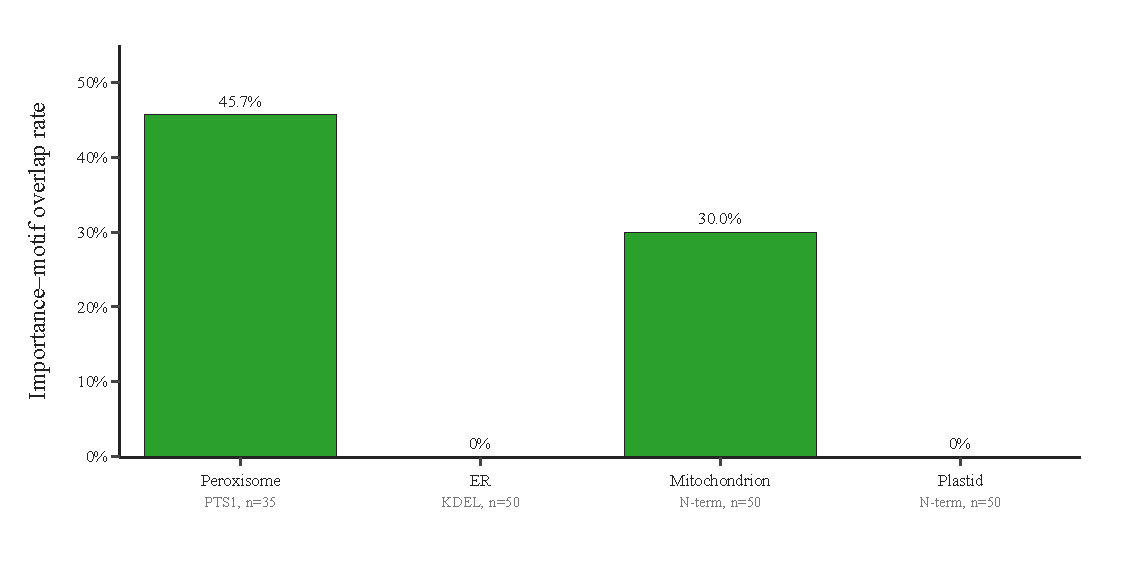
\includegraphics[width=0.82\linewidth]{figures/fig5_motifs.pdf}
  \caption{Importance--motif overlap for the four compartments with
  a canonical short motif. The headline GAT recovers Peroxisome
  PTS1 in $45.7\%$ of explained true positives ($16/35$, Peroxisome's
  small test pool limits $n$) and the mitochondrial N-terminal targeting
  region in $30\%$ ($15/50$). It does \emph{not} recover the ER KDEL
  motif ($0/50$) or plastid N-terminal targeting ($0/50$), even though
  test ROC-AUC for those compartments is high ($0.91$ and $0.99$ resp.).}
  \label{fig:motifs}
\end{figure}

The two positive results are non-trivial: PTS1 is a 3-residue
C-terminal motif and the model is rewarded for ROC-AUC, not for motif
recovery, so a $45.7\%$ overlap rate is meaningful. The mitochondrial
N-terminal positive is similar in spirit. The two null results are
informative as well. The ER KDEL motif sits at the very last 4
residues; if our overlap criterion (top-decile importance overlapping
the regex) is the wrong way to score this, then $0/50$ is a measurement
artefact rather than a model failure. The plastid N-terminal null is
harder to defend: plastid signal peptides are real and N-terminal, and
at least partial recovery was anticipated. We discuss both in
Section~\ref{sec:discussion}.

% =========================================================================
\section{Discussion}\label{sec:discussion}
% =========================================================================

\paragraph{Source of the performance gain.}
The single largest gain in this study comes from the embedding rather
than the graph: frozen ESM2-150M alone, with no graph, no attention,
and no structure, raises macro ROC-AUC from $0.812$ to $0.913$. The graph
adds $\sim\!0.014$ on top. This is consistent with the framing that
ESM2 has already absorbed most of the local sequence regularity and is
exposing it linearly; what the GAT adds is the ability to integrate
that residue-level signal coherently across long-range neighbours, which
shows up most clearly in PR-AUC and F1 (the rare-class metrics) rather
than ROC-AUC.

\paragraph{Sequence versus contact edges.}
Within $0.002$ macro ROC-AUC, sequence-only and contact-only edges are
effectively interchangeable. We interpret this as the GATv2
message-passing being bottlenecked by the richness of the ESM2 features
rather than by the choice of neighbourhood. Combining the two does not improve ROC-AUC
either, but it does improve PR-AUC by $+0.020$ and F1 by $+0.025$,
suggesting that having both edge types lets the rare-class decision
boundary tighten without changing the average ranking quality.

\paragraph{Partial recovery of canonical motifs.}
GNNExplainer recovers PTS1 and mitochondrial N-terminal targeting, the
two motifs whose biological signal is also \emph{positionally local}
in a way that the importance map can hit. It misses ER KDEL and
plastid N-terminal. We do not yet know whether this is a measurement
artefact (the overlap test is too coarse for KDEL's last-4-residue
position) or a model artefact (the GAT is using a non-motif signal for
ER, e.g.\ the surrounding hydrophobic context). Distinguishing these
would require a finer-grained per-residue importance test.

\paragraph{Broader impact.}
Accurate localization predictors aid functional annotation of newly
sequenced proteins and reduce wet-lab triage cost in drug-target
discovery. The risk we see is overconfident predictions on
out-of-distribution proteins (e.g.\ designed sequences with no
homologue), which could mislead downstream wet-lab decisions; the
homology-controlled DeepLoc split protects us during evaluation, but
real deployment would need a calibration audit on held-out organisms.

% =========================================================================
\section{Limitations}\label{sec:limitations}
% =========================================================================

\paragraph{Single-seed training.}
Each ablation row is trained with one random seed (\texttt{--seed 0}).
The eight random-search configurations span a $0.7$ point val ROC-AUC
range, which we interpret as an architectural sensitivity check rather than
a true error bar; a multi-seed estimate would multiply our compute by
$\sim\!5\times$ and was not feasible within the available compute budget.

\paragraph{Fixed contact threshold.}
Rebuilding graphs at multiple $C_\alpha$ thresholds (e.g.\ 6, 8, 10\,\AA)
would triple the structure-stage storage budget and was deferred. The
chosen 8\,\AA{} value is biologically standard but not optimised on val.

\paragraph{AlphaFold-less proteins are dropped.}
The GNN rows train and evaluate on the $\sim\!98\%$ of DeepLoc proteins
that have an AlphaFold prediction; the remaining $\sim\!2\%$ are
excluded. This exclusion introduces a mild small-protein bias (very
short sequences are over-represented among the missing entries), which
we note here so it is not overlooked downstream.

\paragraph{Modest random-search budget.}
Eight configurations is enough to confirm robustness, but not enough to
find a true optimum in the joint hyperparameter space. A larger
search, or Bayesian optimisation over a continuous space, could plausibly
push the headline a further $\sim\!0.01$--$0.02$ in PR-AUC.

\paragraph{Interpretability nulls.}
We report two motif-overlap nulls (ER KDEL, plastid N-terminal) without
diagnosing their cause. Whether the model is (a) using the right
signal but our overlap test is too coarse, or (b) using a different
signal than canonical biology suggests, would require finer-grained
importance analysis (e.g.\ counterfactual ablation of the motif residues
in input).

% =========================================================================
\section{Conclusion}\label{sec:conclusion}
% =========================================================================

A controlled five-row ablation on the DeepLoc~2.0 homology split shows
that, for protein subcellular localization, the dominant lift is
swapping hand features for frozen ESM2 embeddings ($+0.10$ macro
ROC-AUC), with structure-aware graph attention adding a further small
but real gain that is concentrated in PR-AUC and macro F1 on rare
compartments. Sequence and $C_\alpha$ contact edges are
near-interchangeable in isolation but jointly support the best PR-AUC
and F1 under a small random search. GNNExplainer recovers two of four
canonical sorting motifs, validating that the network has learned at
least some real cell biology. Future work should pursue multi-seed
error bars, a finer-grained motif-overlap test, and pretraining
strategies that condition on AlphaFold structure during the embedding
stage rather than only at classifier-time.

\begin{ack}
We thank the DeepLoc~2.0, ESM2, and AlphaFoldDB teams for releasing
their datasets and models. All experiments were carried out on a single
consumer GPU.
\end{ack}

% =========================================================================
\section*{References}
% =========================================================================
{\small
[1] Almagro Armenteros, J.J., Salvatore, M., Emanuelsson, O., et al.\ (2022)
DeepLoc 2.0: multi-label subcellular localization prediction using protein
language models. {\it Nucleic Acids Research} {\bf 50}(W1):W228--W234.

[2] Lin, Z., Akin, H., Rao, R., et al.\ (2023) Evolutionary-scale prediction of
atomic-level protein structure. {\it Science} {\bf 379}(6637):1123--1130. (ESM2)

[3] Jumper, J., Evans, R., Pritzel, A., et al.\ (2021) Highly accurate protein
structure prediction with AlphaFold. {\it Nature} {\bf 596}:583--589.

[4] Varadi, M., Anyango, S., Deshpande, M., et al.\ (2022) AlphaFold Protein
Structure Database: massively expanding the structural coverage of
protein-sequence space. {\it Nucleic Acids Research} {\bf 50}(D1):D439--D444.

[5] Veli\v{c}kovi\'{c}, P., Cucurull, G., Casanova, A., et al.\ (2018) Graph
attention networks. In {\it ICLR}.

[6] Brody, S., Alon, U., \& Yahav, E.\ (2022) How attentive are graph attention
networks? In {\it ICLR}. (GATv2)

[7] Ying, R., Bourgeois, D., You, J., Zitnik, M., \& Leskovec, J.\ (2019)
GNNExplainer: generating explanations for graph neural networks. In
{\it NeurIPS}.

[8] Pedregosa, F., Varoquaux, G., Gramfort, A., et al.\ (2011)
Scikit-learn: machine learning in Python. {\it JMLR} {\bf 12}:2825--2830.

[9] Fey, M.\ \& Lenssen, J.E.\ (2019) Fast graph representation learning with
PyTorch Geometric. In {\it ICLR Workshop on Representation Learning on Graphs
and Manifolds}.
}

% =========================================================================
\appendix

\section{Per-compartment numerical results}

Table~\ref{tab:percomp} lists per-(model, compartment) ROC-AUC for the
five rows that appear in Table~\ref{tab:ablation}. The classical row is
the best-of-three (random forest). All other entries are deterministic
under \texttt{--seed 0}.

\begin{table}[h]
  \caption{Per-compartment test ROC-AUC. Bold marks the per-row best.}
  \label{tab:percomp}
  \centering
  \scriptsize
  \begin{tabular}{lccccc}
    \toprule
    Compartment & Class.\ RF & ESM-MLP & GAT-seq & GAT-cont & GAT-both \\
    \midrule
    Cytoplasm              & 0.747 & 0.845 & 0.868 & \textbf{0.870} & \textbf{0.870} \\
    Nucleus                & 0.812 & 0.906 & 0.921 & \textbf{0.922} & 0.921 \\
    Extracellular          & 0.904 & 0.979 & 0.983 & \textbf{0.984} & 0.983 \\
    Cell membrane          & 0.803 & 0.916 & \textbf{0.925} & 0.925 & 0.923 \\
    Mitochondrion          & 0.837 & 0.945 & \textbf{0.956} & 0.956 & 0.950 \\
    Plastid                & 0.885 & 0.988 & 0.988 & \textbf{0.989} & \textbf{0.989} \\
    Endoplasmic reticulum  & 0.818 & 0.897 & \textbf{0.911} & 0.911 & 0.909 \\
    Lysosome / Vacuole     & 0.750 & 0.856 & 0.866 & \textbf{0.876} & \textbf{0.876} \\
    Golgi apparatus        & 0.680 & 0.832 & \textbf{0.844} & \textbf{0.844} & 0.831 \\
    Peroxisome             & 0.887 & \textbf{0.971} & 0.963 & 0.970 & 0.960 \\
    \midrule
    \emph{Macro mean}      & 0.812 & 0.913 & 0.923 & \textbf{0.925} & 0.921 \\
    \bottomrule
  \end{tabular}
\end{table}

\section{Random-search log}

Table~\ref{tab:sweepfull} shows every configuration tried in the
8-config random search, ordered by validation macro ROC-AUC. The chosen
configuration (id~6) is the best on validation, but the test-set winner
on PR-AUC is config~1, which we did not select, since the test set
was not consulted during model selection.

\begin{table}[h]
  \caption{Random-search configurations and metrics. Selection is on
  val ROC-AUC; test columns are reported for completeness.}
  \label{tab:sweepfull}
  \centering
  \footnotesize
  \begin{tabular}{rccccccc}
    \toprule
    cfg & layers & hidden & heads & dropout & lr & val ROC & test PR \\
    \midrule
    \textbf{6} & 3 & 64  & 8 & 0.0 & $10^{-3}$    & \textbf{0.9094} & 0.6641 \\
    1          & 3 & 128 & 8 & 0.2 & $10^{-3}$    & 0.9085          & \textbf{0.6633} \\
    0          & 3 & 128 & 4 & 0.2 & $3{\cdot}10^{-4}$ & 0.9079          & 0.6476 \\
    4          & 2 & 128 & 8 & 0.2 & $10^{-3}$    & 0.9071          & 0.6496 \\
    3          & 3 & 64  & 8 & 0.2 & $3{\cdot}10^{-4}$ & 0.9072          & 0.6457 \\
    2          & 2 & 128 & 4 & 0.0 & $3{\cdot}10^{-4}$ & 0.9053          & 0.6578 \\
    5          & 2 & 64  & 8 & 0.0 & $3{\cdot}10^{-4}$ & 0.9053          & 0.6246 \\
    7          & 2 & 64  & 4 & 0.2 & $10^{-3}$    & 0.9026          & 0.6310 \\
    \bottomrule
  \end{tabular}
\end{table}

\section{GNNExplainer per-compartment summary}

Of the ten compartments, four have a canonical short motif against
which we can measure overlap quantitatively (Peroxisome PTS1, ER KDEL,
Mitochondrion N-terminal, Plastid N-terminal). The remaining six do
not, and their explanations are released as PNG attribution plots in
\texttt{runs/gnn/explanations/<compartment>/} for qualitative
inspection. Per-compartment overlap counts are in
Table~\ref{tab:explainer}.

\begin{table}[h]
  \caption{GNNExplainer motif-overlap counts on the headline checkpoint.
  $n$ is the number of high-confidence true positives explained;
  ``hits'' is the count whose top-decile node importance overlaps the
  motif region.}
  \label{tab:explainer}
  \centering
  \footnotesize
  \begin{tabular}{lccc}
    \toprule
    Compartment             & $n$ & Hits & Overlap rate \\
    \midrule
    Peroxisome (PTS1)       & 35  & 16   & \textbf{45.7\%} \\
    Mitochondrion (N-term)  & 50  & 15   & \textbf{30.0\%} \\
    Endoplasmic reticulum (KDEL)  & 50 & 0 & 0.0\% \\
    Plastid (N-term)        & 50  & 0    & 0.0\% \\
    \bottomrule
  \end{tabular}
\end{table}

% NeurIPS checklist intentionally omitted from this build.
% Re-enable by uncommenting the line below; the source lives in checklist.tex.
% \section*{NeurIPS Paper Checklist}

\begin{enumerate}

\item {\bf Claims}
    \item[] Question: Do the main claims made in the abstract and introduction accurately reflect the paper's contributions and scope?
    \item[] Answer: \answerYes{}
    \item[] Justification: The abstract and Section~\ref{sec:intro} list four contributions
    (frozen-ESM2 lift, edge-type ablation, GNNExplainer motif validation,
    reproducible Make-driven pipeline), each substantiated by quantitative
    results in Section~\ref{sec:results}.

\item {\bf Limitations}
    \item[] Question: Does the paper discuss the limitations of the work performed by the authors?
    \item[] Answer: \answerYes{}
    \item[] Justification: Section~\ref{sec:limitations} discusses the single-seed
    evaluation, the fixed 8\,\AA{} contact threshold, the loss of
    AlphaFold-less proteins, the modest random search budget, and the failure
    of GNNExplainer to recover ER and plastid motifs.

\item {\bf Theory assumptions and proofs}
    \item[] Question: For each theoretical result, does the paper provide the full set of assumptions and a complete (and correct) proof?
    \item[] Answer: \answerNA{}
    \item[] Justification: The paper is purely empirical and presents no theorems
    or formal claims requiring proof.

\item {\bf Experimental result reproducibility}
    \item[] Question: Does the paper fully disclose all the information needed to reproduce the main experimental results of the paper to the extent that it affects the main claims and/or conclusions of the paper (regardless of whether the code and data are provided or not)?
    \item[] Answer: \answerYes{}
    \item[] Justification: All splits are taken from the public DeepLoc 2.0 release,
    every hyperparameter and the random-search space are listed in
    Section~\ref{sec:experiments}, the chosen headline configuration is given
    in Table~\ref{tab:hyper}, and the entire pipeline is exposed as
    \texttt{make gnn-*} targets with fixed seed (\texttt{--seed 0}).

\item {\bf Open access to data and code}
    \item[] Question: Does the paper provide open access to the data and code, with sufficient instructions to faithfully reproduce the main experimental results, as described in supplemental material?
    \item[] Answer: \answerYes{}
    \item[] Justification: Code is committed to the project repository under
    \texttt{halo/gnn/} and \texttt{halo/spec/}; a \texttt{Makefile} drives every
    stage end-to-end; data are the publicly released DeepLoc~2.0 CSVs and
    AlphaFold structures fetched from AFDB by UniProt accession.

\item {\bf Experimental setting/details}
    \item[] Question: Does the paper specify all the training and test details (e.g., data splits, hyperparameters, how they were chosen, type of optimizer) necessary to understand the results?
    \item[] Answer: \answerYes{}
    \item[] Justification: Section~\ref{sec:experiments} specifies the DeepLoc
    train/val/test partition, the BCE-with-logits loss with positive-class
    re-weighting, the AdamW optimizer with cosine schedule, AMP, batch size,
    epoch budget, and the random-search space over GAT depth, width, heads,
    dropout, and learning rate. Selection is by macro val ROC-AUC; the test
    set is touched once per row.

\item {\bf Experiment statistical significance}
    \item[] Question: Does the paper report error bars suitably and correctly defined or other appropriate information about the statistical significance of the experiments?
    \item[] Answer: \answerNo{}
    \item[] Justification: Each ablation row is trained with a single fixed seed.
    A multi-seed estimate would require roughly $5\times$ the GPU-hours we had
    available on a single laptop RTX~4070 (8\,GB). We instead report
    consistency across the eight random-search configurations
    (Figure~\ref{fig:sweep}), which span a $\sim\!0.7$ point val ROC-AUC range
    and act as an architectural sensitivity check.

\item {\bf Experiments compute resources}
    \item[] Question: For each experiment, does the paper provide sufficient information on the computer resources (type of compute workers, memory, time of execution) needed to reproduce the experiments?
    \item[] Answer: \answerYes{}
    \item[] Justification: All training and explanation runs were performed on a
    single NVIDIA RTX~4070 laptop GPU (8\,GB VRAM); approximate wall-clock
    budgets per stage are given in Section~\ref{sec:experiments}. Total
    project compute is on the order of two GPU-days plus two CPU-evenings of
    AlphaFold downloads and ESM2 caching.

\item {\bf Code of ethics}
    \item[] Question: Does the research conducted in the paper conform, in every respect, with the NeurIPS Code of Ethics?
    \item[] Answer: \answerYes{}
    \item[] Justification: We use only publicly released resources (DeepLoc~2.0,
    ESM2, AlphaFoldDB), perform no human-subjects research, and release no
    high-risk artefacts.

\item {\bf Broader impacts}
    \item[] Question: Does the paper discuss both potential positive societal impacts and negative societal impacts of the work performed?
    \item[] Answer: \answerYes{}
    \item[] Justification: A brief broader-impacts paragraph in
    Section~\ref{sec:discussion} notes the positive value of accurate
    localization predictors in functional annotation and drug-target
    triage, and the risk that overly confident predictions on
    out-of-distribution proteins (e.g.\ designed sequences) could mislead
    downstream wet-lab decisions.

\item {\bf Safeguards}
    \item[] Question: Does the paper describe safeguards that have been put in place for responsible release of data or models that have a high risk for misuse?
    \item[] Answer: \answerNA{}
    \item[] Justification: We release a small classifier head on top of frozen
    public embeddings; the artefact has no plausible misuse path and poses no
    high-risk dual-use concern.

\item {\bf Licenses for existing assets}
    \item[] Question: Are the creators or original owners of assets used in the paper properly credited and are the license and terms of use explicitly mentioned and properly respected?
    \item[] Answer: \answerYes{}
    \item[] Justification: DeepLoc~2.0 (academic use), ESM2 (MIT licence),
    AlphaFoldDB (CC-BY 4.0), \texttt{torch\_geometric} (MIT), and
    \texttt{scikit-learn} (BSD-3) are cited in
    Section~\ref{sec:related} and Section~\ref{sec:experiments}.

\item {\bf New assets}
    \item[] Question: Are new assets introduced in the paper well documented and is the documentation provided alongside the assets?
    \item[] Answer: \answerNA{}
    \item[] Justification: The paper does not release a new dataset or pretrained
    model. The trained GAT checkpoint and the GNNExplainer attributions are
    project artefacts retained in the repository for reproducibility but are
    not packaged as a public release.

\item {\bf Crowdsourcing and research with human subjects}
    \item[] Question: For crowdsourcing experiments and research with human subjects, does the paper include the full text of instructions given to participants and screenshots, if applicable, as well as details about compensation (if any)?
    \item[] Answer: \answerNA{}
    \item[] Justification: The work involves no crowdsourcing and no human subjects.

\item {\bf Institutional review board (IRB) approvals or equivalent for research with human subjects}
    \item[] Question: Does the paper describe potential risks incurred by study participants, whether such risks were disclosed to the subjects, and whether Institutional Review Board (IRB) approvals (or an equivalent approval/review based on the requirements of your country or institution) were obtained?
    \item[] Answer: \answerNA{}
    \item[] Justification: The work involves no human subjects and therefore did
    not require IRB review.

\item {\bf Declaration of LLM usage}
    \item[] Question: Does the paper describe the usage of LLMs if it is an important, original, or non-standard component of the core methods in this research?
    \item[] Answer: \answerYes{}
    \item[] Justification: The frozen ESM2-150M protein language model is a core
    component of the feature extractor and is described in
    Section~\ref{sec:method}. No general-purpose LLM is used in the core
    methodology; LLM-assisted writing was limited to copy-editing.

\end{enumerate}


\end{document}
